\documentclass[12pt,a4paper,openright,twoside]{book}
\usepackage[utf8]{inputenc}
\usepackage{disi-thesis}
\usepackage{code-lstlistings}
\usepackage{notes}
\usepackage{shortcuts}
\usepackage{acronym}

\school{\unibo}
\programme{MSc in Engineering and Computer Science}
\title{Feasibility of Reactive Aggregate Programming via Kotlin Flows}
\author{Filippo Vissani}
\date{\today}
\subject{Laboratory of Software Systems}
\supervisor{Prof. Danilo Pianini}
\cosupervisor{Dott. Gianluca Aguzzi}
\session{IV}
\academicyear{2022-2023}

% Definition of acronyms
\acrodef{IoT}{Internet of Thing}
\acrodef{vm}[VM]{Virtual Machine}
\acrodef{jvm}[JVM]{Java Virtual Machine}

\mainlinespacing{1.241}

\begin{document}

\frontmatter\frontispiece

\begin{abstract}	
% Max 2000 characters, strict.
% Very brief (e.g. 250-300 words)
% Abstract should briefly point out: Context, Problem/Objectives, Methods/Contribution, Results, Conclusions
\end{abstract}

\begin{dedication} % this is optional
Optional. Max a few lines.
\end{dedication}

\begin{acknowledgements} % this is optional
Optional. Max 1 page.
\end{acknowledgements}

%----------------------------------------------------------------------------------------
\tableofcontents
\listoffigures     % (optional) comment if empty
\lstlistoflistings % (optional) comment if empty
%----------------------------------------------------------------------------------------

\mainmatter

%----------------------------------------------------------------------------------------
\chapter{Introduction}
\label{chap:introduction}
%----------------------------------------------------------------------------------------

% Introduction should set: Context, Scope, Significance (Motivation), Goals/High-level Questions, Methodology (briefly), Organization of the paper (chapters and what they include)

%----------------------------------------------------------------------------------------
\chapter{Background}
\label{chap:background}
%----------------------------------------------------------------------------------------

This chapter provides a broad overview of the concepts, paradigms, and frameworks that served as points of reference during the entire development of this thesis.

\section{Functional Programming}

The functional paradigm, in the context of computer science, involves building programs through the application and composition of functions. It adopts a declarative approach, where function definitions are represented as trees of expressions mapping values to other values, rather than relying on a sequence of imperative statements to update the program's running state.

\subsection{Concepts}

This section elucidates fundamental concepts that form the basis of functional programming.

\paragraph{Higher-order functions}

Higher-order functions possess the ability to either receive functions as arguments or produce them as results. The nuanced difference lies in the mathematical concept denoted by "higher-order", which involves functions operating on other functions.

These functions facilitate partial application or currying, enabling a technique where a function is applied to its arguments one at a time. With each application, a new function is created to handle the next argument. This approach allows programmers to express ideas succinctly, such as representing the successor function by partially applying the addition operator to the natural number one.

\paragraph{Purity}
Pure functions, or expressions, lack side effects. This absence of side effects endows pure functions with various advantageous properties, many of which can be leveraged for code optimization. A pure function, to be defined as such, must meet the following properties:

\begin{itemize}
    \item If the result of a pure expression is not used, it can be removed without influencing other expressions.
    \item If a pure function is invoked with arguments that do not introduce side effects, the result remains constant concerning that set of arguments. Repeatedly calling the pure function with the same arguments yields identical results.
\end{itemize}

\paragraph{Recursion}

Functional languages typically employ recursion for iteration. Recursive functions call themselves, allowing an operation to iterate until it meets the base case. Generally, recursion involves managing a stack, consuming space proportional to the recursion depth. This characteristic might render recursion less favorable compared to imperative loops due to potential space inefficiency. Nonetheless, a specific type of recursion called tail recursion can be identified and optimized by a compiler, producing code similar to that used for iteration in imperative languages. Implementing tail recursion optimization involves transforming the program using a continuous passing style during compilation.

\paragraph{Evaluation strategies}

In functional languages, various methods are commonly provided for evaluating arguments during their passage to functions. Three primary approaches include:

\begin{itemize}
    \item \textit{Call-by-value}: This involves evaluating arguments before the function application.
    \item \textit{Call-by-name}: Here, arguments are assessed each time their value is needed within the function body.
    \item \textit{Call-by-need}: Also known as lazy evaluation, this approach involves evaluating arguments only when their value is first required within the function body.
\end{itemize}

\paragraph{Type systems}

Functional programming languages have leaned towards employing typed lambda calculus. This approach involves rejecting all invalid programs at compilation time, even at the risk of encountering false positive errors. In contrast, untyped lambda calculus, accepts all valid programs at compilation time, running the risk of false negative errors, as it rejects invalid programs only at runtime when there is sufficient information to distinguish valid from invalid programs. The incorporation of algebraic data types enhances the ease of manipulating complex data structures. Additionally, the robust compile-time type checking contributes to program reliability, offering a level of assurance even in the absence of other reliability techniques. Furthermore, type inference alleviates the need for manual declaration of types by the programmer in most cases.

\paragraph{Referential transparency}

In functional programming, there are no assignment statements; once a variable is defined, its value remains constant throughout the program's execution. This characteristic eliminates the possibility of side effects since any variable can be substituted with its actual value at any given point in the program. Consequently, functional programs are characterized by referential transparency.

\paragraph{Data structures}

Purely functional data structures are often represented differently from their imperative counterparts. While arrays, providing constant access and update times, are fundamental in most imperative languages, purely functional alternatives might employ maps or random access lists. Although these alternatives allow for a purely functional implementation, they come with logarithmic access and update times. One distinguishing feature of purely functional data structures is persistence, which involves maintaining unmodified previous versions of the data structure.

\subsection{Functional Programming in Kotlin}

Kotlin, an open-source programming language characterized by static typing, accommodates both object-oriented and functional programming paradigms. Rather than striving for uniqueness, Kotlin derives inspiration from decades of language development. Variants of Kotlin are designed to target different platforms, including the \ac{jvm}, JavaScript, and native code.

In Kotlin, functions are treated as first-class entities, implying their ability to be stored in variables and data structures. Additionally, they can be passed as arguments to and returned from other higher-order functions. The operations that can be performed on functions are equivalent to those applicable to other non-function values.

To support these functionalities, Kotlin, being a statically typed programming language, employs a family of function types to represent functions. Moreover, it incorporates specialized language constructs, such as lambda expressions.

An illustrative instance of a higher-order function in Kotlin is the functional programming idiom \texttt{fold} (\cref{lst:fold-function})
employed for collections. This function receives an initial accumulator value and a combining function. Subsequently, it constructs its return value by iteratively combining the current accumulator value with each element in the collection. Importantly, the accumulator value is replaced with each iteration.

\lstinputlisting[float,language=Kotlin,label={lst:fold-function},caption= \texttt{fold} function]{listings/fold.kt}

the \texttt{combine} parameter has the function type \((R, T) \rightarrow R\), so it accepts a function that takes two arguments of types \textit{R} and \textit{T} and returns a value of type \textit{R}. It is invoked inside the \texttt{for} loop, and the return value is then assigned to \texttt{accumulator}.

Kotlin uses function types, such as \((Int) \rightarrow String\), for declarations that deal with functions. Each function type in Kotlin is characterized by a parenthesized list specifying the parameter types and a return type. For example, \((A, B) \rightarrow C\) represents a type indicative of functions that accept two arguments of types \textit{A} and \textit{B}, yielding a result of type \textit{C}. The parameter list may be empty, denoted by \(() \rightarrow A\). It is essential to note that the return type cannot exclude the declaration of \texttt{Unit}. Function types have the option to include an additional receiver type, indicated before the dot in the notation. For instance, the type \(A.(B) \rightarrow C\) signifies functions that can be invoked on a receiver object \textit{A}, accepting a parameter \textit{B}, and producing a result of type \textit{C}.

\section{Reactive Programming}

Reactive programming is a declarative programming paradigm centered around data streams and the propagation of changes. Within this framework, expressing both static and dynamic data streams becomes straightforward. Additionally, the paradigm allows for the indication of inferred dependencies in the associated execution model, enabling the automatic propagation of alterations in the data flow.

\subsection{Callback Pattern}

Reactive programming is grounded in the principle of asynchronous event processing, wherein events are handled without impeding the processing of concurrent events. Unlike synchronous procedure calls, where the program flow halts until the procedure returns the result, asynchronous communication involves the caller registering a \textit{callback procedure} procedure to be invoked upon result availability. The caller, unburdened by waiting for the result, can proceed with other tasks. In essence, the asynchronous procedure receives not only the necessary parameters but also instructions regarding the subsequent actions upon result availability, thus incorporating a forward-looking aspect into the invocation. Additionally, the caller has the flexibility to register multiple callback procedures, a valuable feature for scenarios necessitating notifications for both success and failure outcomes. The widely adopted implementation of the \textit{callback pattern} (\cref{fig:callback-pattern}) in object-oriented programming involves the Observer pattern. Here, the return value of the asynchronous procedure call is defined \textit{observable}, while the \textit{callback procedure} assumes the role of the \textit{observer}.

\begin{figure}
    \centering
    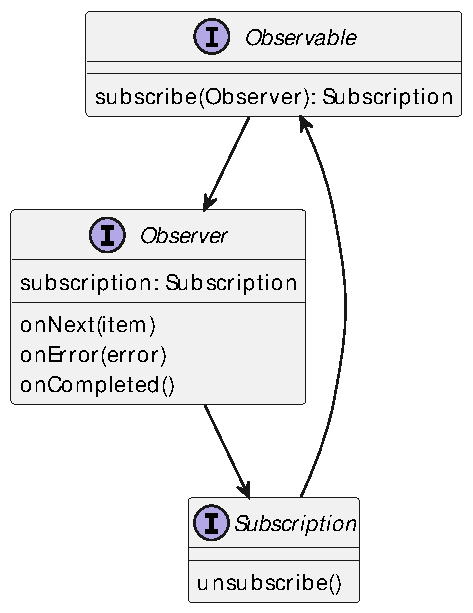
\includegraphics[width=.5\linewidth]{figures/callback-pattern.pdf}
    \caption{Callback pattern: class diagram}
    \label{fig:callback-pattern}
\end{figure}

In the context of reactive applications, the mere handling of a singular event is insufficient. Rather, the application is required to manage a continuous stream of events. In the realm of reactive streams, the \texttt{Observable} represents not merely an isolated event but an ongoing sequence of events. Subsequently, the \texttt{Observer} is tasked with furnishing callbacks for both successful and unsuccessful outcomes, as well as for the termination of the event stream.

\subsection{Back pressure}

Divergence exists among reactive streams concerning how the flow of the stream is regulated. Two distinct approaches, namely push and pull, are identified. In the push paradigm, the consumer lacks precise knowledge of when a new event will be emitted. Consequently, the consumer is susceptible to being inundated by the unceasing stream of events. To mitigate this, the consumer must possess the capability to exert control over the stream's flow, a concept referred to as \textit{back pressure}. Conversely, in the pull paradigm, the consumer explicitly determines when to retrieve the subsequent event from the stream.

\subsection{Reactive Operators}

The primary advantage offered by libraries furnishing the reactive streams APIs lies in the provision of operators. These operators are essentially functions applicable to a data stream, adept at solving problems related to the processing of reactive streams, encompassing tasks such as filtering, mapping (\cref{fig:reactive-map}), and aggregating.

Furthermore, these operator functions are intentionally designed to be composable, signifying their capability to be consecutively linked to construct processing pipelines. Each operator function receives an observable as input and yields another observable as output. Consequently, the outcome of one operator function can seamlessly serve as the input for another operator function, a concept termed operator chaining.

\subsection{Hot and Cold Observables}

The start of emission of data for an observable depends on its nature. In the case of a \textit{hot observable}, the emission of items may start immediately upon its creation. Consequently, any subsequent observer subscribing to this observable may commence observation at any point within the sequence, potentially in the middle. Conversely, a \textit{cold observable} adopts a different approach by deferring emission until an observer subscribes to it. In this scenario, the observer is assured of obtaining the entire sequence from its inception once the subscription is initiated.

This dichotomy between hot and cold observables reflects a fundamental distinction in their behavior, influencing the temporal aspect of data emission and subsequent observation by observers. The inherent characteristics of each type contribute to varying scenarios and considerations when designing and utilizing observables in reactive programming contexts.

\begin{figure}
    \centering
    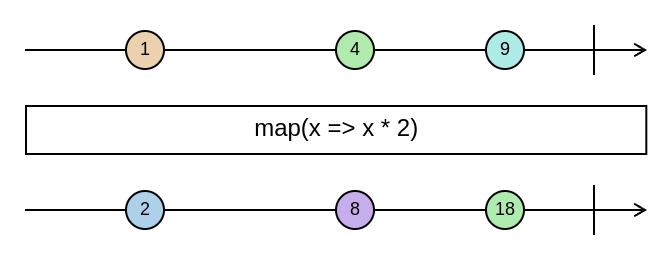
\includegraphics[width=\linewidth]{figures/map-marble.png}
    \caption{Map operator in reactive applications}
    \label{fig:reactive-map}
\end{figure}

\subsection{Reactive Programming in Kotlin}

Kotlin\footnote{\url{https://kotlinlang.org/}} Flow\footnote{\url{https://kotlinlang.org/docs/flow.html}} is a library for handling asynchronous data streams, providing a sequential emission of values that can be completed normally or with an exception. The key distinction lies in its cold flow property, where intermediate operators like \texttt{map}, \texttt{filter}, \texttt{take}, and \texttt{zip} set up a chain of operations for future execution without executing any code immediately, showcasing the asynchronous nature of flows. Terminal operators, such as \texttt{collect}, \texttt{single}, \texttt{reduce}, and \texttt{toList}, trigger the execution of all operations in a suspending manner, completing either normally or exceptionally based on the success or failure of upstream flow operations. By default, flows are sequential, with exceptions for specific operations like \texttt{buffer} and \texttt{flatMapMerge} that introduce concurrency. The \texttt{Flow} interface doesn't inherently differentiate between cold and hot streams, but a \texttt{SharedFlow} subtype and operators like \texttt{stateIn}, \texttt{shareIn}, and \texttt{produceIn} enable the transformation of any flow into a hot stream, allowing for repeated collections or emitting different values from the same running source on each collection.

The example \cref{lst:flow-example} demonstrates the asynchronous nature of Kotlin Flow and how it allows concurrent execution without blocking the main thread. The \texttt{simple} function creates a flow using the \texttt{flow} builder. Inside the flow, it emits values from one to three with a delay of one hundred milliseconds between each emission. The delay simulates an operation that takes time, such as network calls or disk I/O. In the \texttt{main} function, a coroutine is launched using \texttt{launch} to run concurrently with the main thread. This coroutine prints messages indicating that it's not blocked and introduces delays between each message. As the flow is collected in the main coroutine, the emitted values are printed and interleaved with the messages from the concurrent coroutine (\cref{lst:flow-example-result}). This demonstrates that the main thread is not blocked during the execution of the flow, thanks to the asynchronous nature of flows.

\lstinputlisting[float,language=Kotlin,label={lst:flow-example},caption=Kotlin Flow example]{listings/flow-example.kt}

\lstinputlisting[float,label={lst:flow-example-result},caption=Kotlin Flow example result]{listings/flow-example-result.txt}

\section{Aggregate Programming}

\subsection{Field Calculus}

\subsection{Abstractions}

% Context
% Sensors
% Neighbor
% Path
% Slot
% Export

\subsection{Proactive Model}

% talk about semantics

\subsection{Reactive Model}

% talk about semantics

%----------------------------------------------------------------------------------------
\chapter{Analysis}
\label{chap:analysis}
%----------------------------------------------------------------------------------------
\section{State of the Art}

\subsection{Protelis}

\subsection{ScaFi}

\subsection{Collektive}

\subsection{FCPP}

\subsection{FRASP}

\section{Design of FRASP}

% talk about constructs and semantics

\section{Design of Collektive}

% talk about constructs and semantics

\section{Integration of FRASP in Collektive}

%----------------------------------------------------------------------------------------
\chapter{Design}
\label{chap:design}
%----------------------------------------------------------------------------------------

\section{Architecture}

\subsection{Purely Reactive Model}

\subsection{Model with Reactive Messages and Sensors}

\section{Detailed Design}

\subsection{Purely Reactive Model}

\subsection{Model with Reactive Messages and Sensors}

%----------------------------------------------------------------------------------------
\chapter{Implementation}
\label{chap:implementation}
%----------------------------------------------------------------------------------------

\section{Purely Reactive Model}

\section{Model with Reactive Messages and Sensors}

\chapter{Evaluation}
\label{chap:evaluation}
%----------------------------------------------------------------------------------------

\section{Analysis of the Ergonomics of the Proposed Models}

\subsection{Purely Reactive Model}

\subsection{Model with Reactive Messages and Sensors}

\section{Testing}

%----------------------------------------------------------------------------------------
\chapter{Conclusion}
\label{chap:conclusion}
%----------------------------------------------------------------------------------------

% Conclusion chapter should point out: (1) Briefly recall problem, starting point and methods adopted, (2) Briefly report Findings, (3) Briefly discuss benefits/limitations, (4) Discuss Future Work

%----------------------------------------------------------------------------------------
% BIBLIOGRAPHY
%----------------------------------------------------------------------------------------

\backmatter

\nocite{*} % comment this to only show the referenced entries from the .bib file

\bibliographystyle{alpha}
\bibliography{bibliography}

\end{document}